\chapter{Descripción del diseño de la base de datos}\label{chapter:database}
El desarrollo de la informática y la computación ha permitido
el almacenamiento de grandes cantidades de datos en espacios 
físicos limitados. Actualmente los sistemas de bases de datos juegan
un papel fundamental en el desarrollo de todo tipo de sistemas computacionales.

El diseño de base de datos es un proceso fundamental a la hora 
de modelar el conjunto de datos y las operaciones que se deseen
realizar sobre ellos. Un correcto diseño de la base de datos
es esencial para garantizar la consistencia de la información,
eliminar datos redundantes, ejecutar consultas de manera 
eficiente y mejorar el rendimiento de la base de datos [\cite{db_book_cap2}]. 

\section{Metodología de diseño de bases de datos}
La complejidad de la información y la cantidad de requisitos que se 
deseen modelar en un sistema computacional hacen que el diseño de una 
base de datos no sea una tarea sencilla. Por tanto es común es común 
descomponer el proceso de diseño en tres etapas fundamentales: diseño conceptual,
diseño lógico y diseño físico. 


\subsection{Diseño conceptual}
En esta fase se obtiene como resultado una representación 
abstracta y de alto nivel de la realidad a partir de las 
especificaciones de requisitos de usuario [REF libro]. El diseño
conceptual comienza con la identificación de las necesidades de los 
usuarios, que a menudo se pueden obtener a través de: examinar
la documentación existente como formularios, observando y
analizando el procesamiento de la información en el proceso que 
se desea modelar o mediante entrevistas a los usuarios finales [\cite{db_requirement_analysis}].

El objetivo del diseño conceptual es describir el contenido de 
información de la base de datos, mediante un esquema conceptual de
la base de datos [\cite{db_book_cap3}], que es independiente del SGBD
que se utilice para manipular la base de datos.
Los programadores o diseñadores utilizan modelos conceptuales de datos 
para la construcción de esquemas. El modelo entidad-relación es uno 
de los más utilizados para el diseño conceptual de bases de datos. Fue 
introducido por Peter Chen en 1976 [REF], y está formado por 
un conjunto de conceptos que permiten describir la realidad mediante 
representaciones gráficas y lingüísticas.

La metodología utilizada 
para el desarrollo del modelo conceptual de datos para la modelación 
de los procesos de asignación de docencia y confección de tribunales de 
tesis fue la metodología genérica MER/XX, que se basa en un enfoque
híbrido entre el modelo entidad/relacional extendido y los conceptos de la 
modelación orientada a objetos [\cite{db_book_cap2}]. 

El modelo entidad-relación extendido describe con un alto nivel de abstracción
el significado de los datos, las relaciones entre ellos y las reglas de negocio 
de un sistema de información. Sus dos elementos principales son las entidades y 
las relaciones, además existen extensiones al modelo básico 
como atributos de las entidades o cardinalidades de las relaciones, 
que aportan al modelo una mayor expresividad.



\subsection{Diseño lógico}
Es el proceso de transformar el esquema conceptual del dominio de la aplicación
que se obtiene en la fase anterior,
en un esquema para el modelo de datos subyacente a un SGBD particular.
Existen diferentes modelos matemáticos utilizados para el diseño lógico
de las bases de datos, tales como: el modelo de listas invertidas[REF], el modelo 
jerárquico[REF], el modelo de redes[REF] y el modelo relacional[REF]. 

El modelo relacional fue propuesto por Edgar Frank Codd en 1970. Es un 
modelo que se basa en la lógica de predicados y en la teoría 
de conjuntos, donde todos los datos se representan en términos de tuplas, 
agrupados en relaciones.

El modelo relacional fue el primer modelo de base de datos que se describió en términos 
matemáticos formales. A pesar de que existen  
implementaciones del modelo de base de datos relacional como lo definió originalmente 
Codd, no han tenido éxito popular hasta el momento. No obstante al modelo relacional se le 
atribuye un gran valor por su desarrollo teórico, que ha sido fundamento de muchos de los 
sistemas de gestión de bases de datos relacionales que se utilizan hoy en la actualidad, como:
MySQL, Oracle, SQL Server, PostgreSQL y Microsoft Access. 

El resultado de esta fase consiste en una descripción de las estructuras 
de datos utilizadas para almacenar la base de datos[\cite{db_book_cap3}], que se 
ajuste al modelo que utilice el SGBD. Esto quiere decir que,
si el modelo conceptual es expresado como un modelo 
entidad-relación y el modelo lógico utilizado en el SGBD es el modelo 
relacional, entonces las entidades, relaciones y los atributos del modelo entidad-relación
deben representarse como relaciones. 

NOTA: ACLARAR el concepto de relación en el modelo relacional


% El objetivo del diseño de bases de datos lógicas es crear 
% tablas bien estructuradas que reflejen adecuadamente el 
% entorno empresarial de la empresa.

\subsection{Diseño físico}
En esta etapa se transforma la estructura obtenida en la etapa del diseño
lógico, con el objetivo de conseguir mayor eficiencia. Es necesario
evaluar los aspectos de implementación física relacionados al SGBD que se utilice.
Por ejemplo: si se trabaja con una base de datos relacional, la 
transformación de la estructura puede consistir en crear una nueva relación que 
sea la combinación de varias relaciones o separar una relación en varias relaciones o 
añadir algún atributo calculable a una relación. \\




% Para el almacenamiento de los datos hizo uso de SQLite 3
% como sistema de gestión de bases de datos relacionales,
% el cual viene integrada en Django por defecto.

\section{Correcto diseño de bases de datos relacionales}

El diseño de una base de datos mediante el enfoque relacional, es una 
tarea no determinista, es posible obtener distintos esquemas relacionales 
como propuestas de la base de datos.
Un diseño incorrecto de una base de datos puede no responder apropiadamente a las exigencias
del proceso que se modela, y puede conllevar a la generación de dificultades o 
errores en el acceso a los datos. Entre los principales errores o dificultades que se pueden generar
se encuentran:

\begin{itemize}
    \item \textbf{Redundancia en los datos}, provoca un aumento innecesario 
    del tamaño de la base de datos, disminuyendo la eficiencia, además puede provocar 
    inconsistencia de los datos que puede conducir a la corrupción de los mismos. 
    \item \textbf{Violación de la integridad de los datos}, el término ``integridad de los datos'' se 
    refiere a la correctitud y completitud de la información en una base de datos. Cuando los datos son 
    modificados con sentencias INSERT, DELETE o UPDATE la integridad de los datos puede comprometerse.
\end{itemize}



Para lograr un correcto diseño de la base de datos se recomienda aplicar un método formal de 
análisis a cada uno de los esquemas obtenidos intuitivamente durante la fase de diseño conceptual, 
que se conoce como proceso de normalización.

\subsection{Normalización}
La normalización de una base de datos es un proceso que consiste 
en aplicar una serie de reglas a las relaciones obtenidas 
tras el paso del modelo entidad-relación (diseño conceptual) al modelo 
relacional (diseño lógico), con el objetivo de minimizar la redundancia de datos.
Cada regla se denomina una ``forma normal'', si se cumple la primera regla, se dice que 
la base de datos está en ``primera forma normal'', si se cumplen las tres 
primeras reglas se dice que la base de datos está en ``tercera forma normal''. El proceso de 
normalización se puede caracterizar como la transformación sucesiva de una colección de 
relaciones hacia una forma más restrictiva, de modo que mientrás mas profundo sea el nivel 
de normalización menor será la redundancia que albergue la base de datos [\cite{db_book_cap4}].
A continuación se introducen las definiciones de las reglas formales:

\begin{itemize}
    \item \textbf{Primera Forma Normal (1FN)}: una relación está en 1FN si y solo si, para 
    cada ocurrencia de la relación, toda tupla contiene exactamente un valor del dominio subyacente en
    cada atributo.
    \item \textbf{Segunda Forma Normal (2FN)}: una relación está en 2FN si, además de estar en 
    1FN, todos los atributos que no forman parte de alguna llave candidata constituyen información 
    acerca de la(s) llave(s) completa(s) y no de algún subconjunto de ella(s).
    \item \textbf{Tercera Forma Normal (3FN)}: una relación está en 3FN si, además de estar en 2FN,
    los atributos que no forman parte de alguna llave candidata constituyen información solo acerca
    de la(s) llave(s) y no acerca de otros atributos.
\end{itemize}


Aunque existen otros niveles de normalización como la ``Forma Normal de Boyce-Codd (BCFN)'',
la ``Cuarta Forma Normal(4FN)'' y la ``Quinta Forma Normal (5FN)'',
se considera que una base de datos en 3FN presenta niveles nulos o 
admisibles de redundancia en los datos[\cite{ws_3FN}].





% Para la implementación del sistema de gestión es necesario el almacenamiento
% y procesamiento de los datos que intervienen en los procesos de asignación de 
% docencia y confección de tribunales de tesis. A continuación se brinda una 
% descripción de cómo se modelaron estos procesos.

\section{Modelación de la asignación de docencia}
En la fase de diseño conceptual se modelaron las entidades fundamentales
que intervienen en el proceso de la asignación de docencia, 
así como las interrelaciones que se establecen entre ellas
y se obtuvo el siguiente
esquema a partir del modelo entidad-relación extendido.

\begin{figure}[H]
    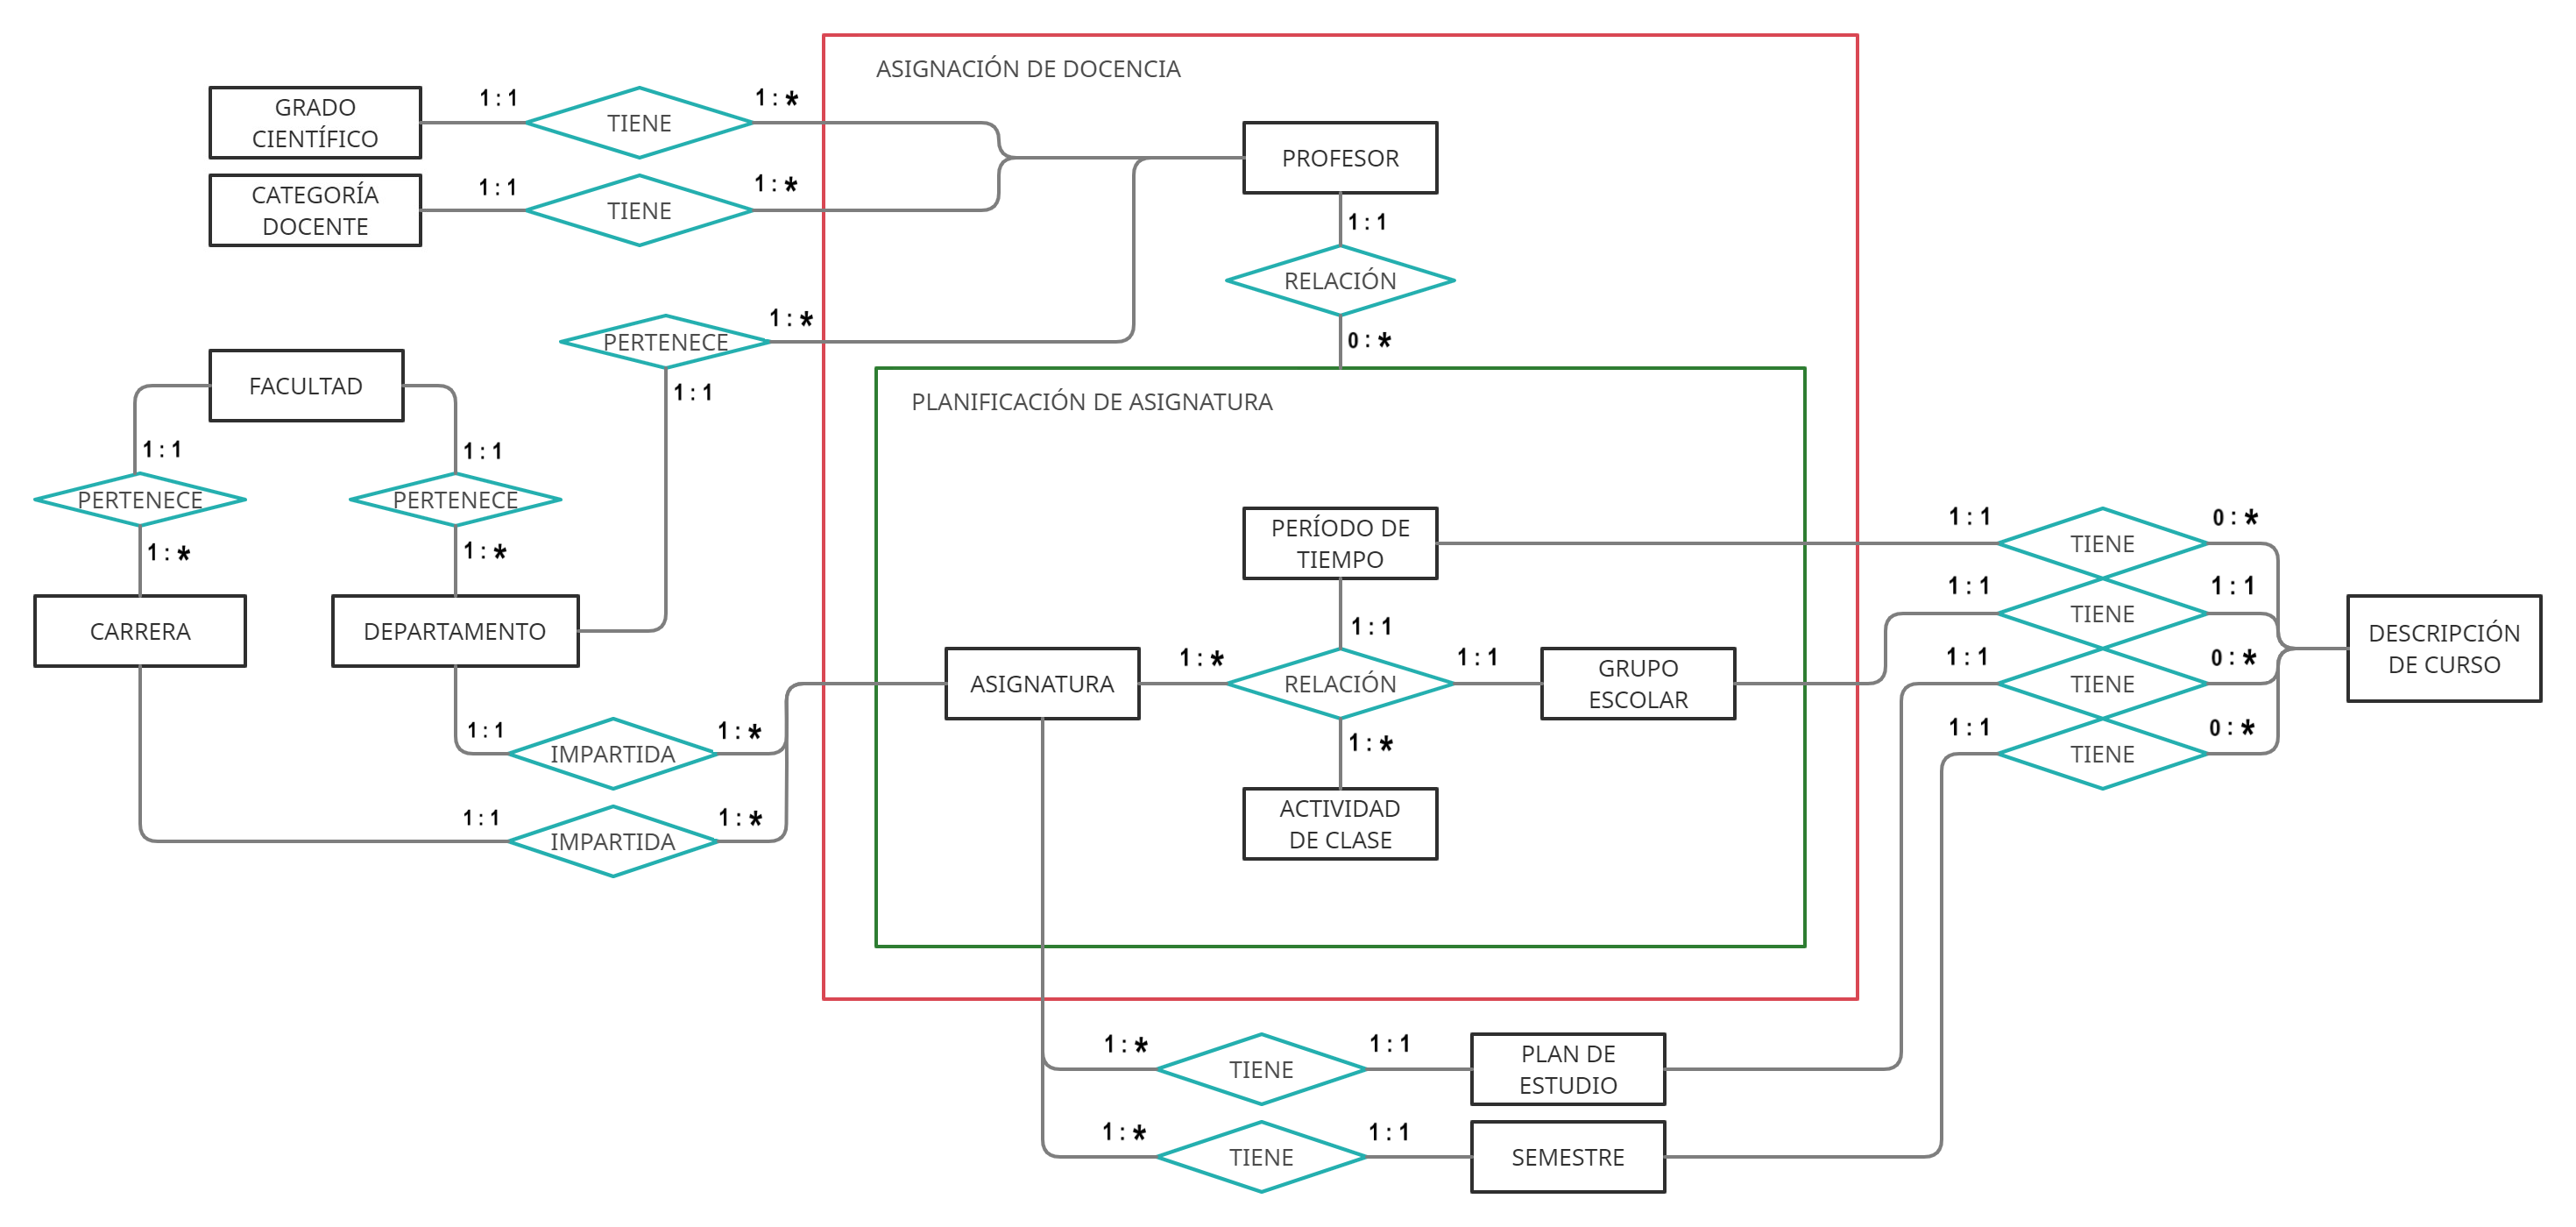
\includegraphics[scale=0.2]{Graphics/Database/MERXX-TA-FINAL.png}
\end{figure}


Con el objetivo de simplificar la representación del modelo entidad-relación
no se agregaron a la imagen los atributos correspondientes a cada entidad, por lo 
que a continuación se describen las entidades en mayor profundidad.


\subparagraph{FACULTAD:}
Representa las facultades de la Universidad de La Habana.
El nombre de la facultad se modela como un atributo, mientras que 
las carreras que se estudian en la facultad y los departamentos que pertenecen 
a ella, se modelan como relaciones con las entidades CARRERA y DEPARTAMENTO, respectivamente.
Una facultad tiene uno o muchos departamentos, y en 
una facultad se pueden estudiar una o más carreras.

\subparagraph{CARRERA:}
Representa las carreras que se estudian en la Universidad de La Habana.
El nombre de la carrera se modela como un atributo, mientras que la facultad a la que pertenece la carrera y
las asignaturas que se imparten en ella, se modelan como relaciones con las entidades FACULTAD y
ASIGNATURA, respectivamente. 
Una carrera pertenece a una única facultad y en una carrera se imparten una o muchas asignaturas.

\subparagraph{DEPARTAMENTO:}
Representa los departamentos de una facultad de la Universidad de La Habana.
El nombre del departamento se modela como un atributo, mientras que los profesores que 
pertenecen a un departamento, las asignatura que son atendidas por el departamento y la 
facultad a la que pertenece el departamento, se modelan como relaciones con las entidades 
PROFESOR, FACULTAD y ASIGNATURA, respectivamente. Un departamento pertenece a una única facultad,
un departamento atiende una o muchas asignaturas y a un departamento pertenecen uno o muchos 
profesores.

\subparagraph{PROFESOR:}
Agrupa los datos asociados a los profesores.
Los campos nombre y apellidos se modelan como atributos,  
mientras que, la categoría docente, el grado 
científico de un profesor y el departamento al que pertenece, se modelan como 
relaciones con las entidades CATEGORÍA DOCENTE, GRADO CIENTÍFICO y 
DEPARTAMENTO, respectivamente. Un profesor pertenece a un único departamento y puede tener solo 
un grado científico y una categoría docente. 


\subparagraph{CATEGORÍA DOCENTE:}
Representa la categoría docente que tienen los profesores.
El nombre de la categoría docente se modela como un atributo. 
Pueden existir uno o muchos profesores con una misma categoría docente.

\subparagraph{GRADO CIENTÍFICO:}
Representa el grado científico que tienen los profesores.
El nombre del grado científico se modela como un atributo.
Pueden existir uno o muchos profesores con un mismo grado científico.





\subparagraph{ASIGNATURA:}
Agrupa los datos asociados a las asignaturas.
Los campos nombre de la asignatura y cantidad de horas 
totales a impartir, se modelan como atributos, mientras que
el plan de estudio asociado a la asignatura, el semestre en el que se 
imparte, el departamento responsable de la asignatura y la carrera a la 
que pertenece, se modelan como relaciones con las entidades
PLAN DE ESTUDIO, SEMESTRE, DEPARTAMENTO y CARRERA respectivamente. Una asignatura 
es atendida por un único departamento, pertenece a una única carrera, se imparte en un 
único semestre y tiene un único plan de estudio. Las asignaturas que se imparten de forma 
anual son representadas como dos asignaturas independientes.

\subparagraph{PLAN DE ESTUDIO:}
Representa el plan de estudio por el que se rige una asignatura.
El nombre del plan de estudio se modela como un atributo.
Pueden existir una o muchas asignaturas con el mismo plan de estudio.



\subparagraph{SEMESTRE:}
Representa los semestres asociados a una carrera. 
El nombre del semestre se modela como un atributo.
Pueden existir una o muchas asignaturas que se imparten en 
el mismo semestre. 


\subparagraph{PERÍODO DE TIEMPO:}
Representa los períodos de tiempo del año.
El nombre del período de tiempo se modela como un atributo.
Pueden existir una o muchas asignaturas que se imparten en 
el mismo período de tiempo.


\subparagraph{GRUPO ESCOLAR:}
Representa los años académicos asociados a una carrera, como por ejemplo:
Matemática primer año (M1) o Computación tercer año (C3).
El nombre del grupo escolar se modela como un atributo.

\subparagraph{ACTIVIDAD DE CLASE:}
Representa los tipos de actividades que se imparten en una asignatura, 
tales como: conferencias, clases prácticas, seminarios, laboratorios, otros. 

\subparagraph{PLANIFICACIÓN DE ASIGNATURA:}
Se crea con el objetivo de modelar la separación de una asignatura
según las actividades de clases a impartir, en un período de tiempo y para
un grupo escolar específico. Está compuesta por la agregación de las entidades ASIGNATURA, ACTIVIDAD DE CLASE, GRUPO 
ESCOLAR y PERÍODO DE TIEMPO.
Se agregan los atributos cantidad de horas para el tipo de actividad a realizar y 
la cantidad de grupos.
Por ejemplo (poner ejemplo real de una asignatura
con distintas act de clase y como queda la separación)



% Entidad creada con el objetivo de separar las distintas actividades 
% que se imparten en una asignatura ( conferencia, clases 
% prácticas, seminarios, laboratorios, otras )  para
% realizar la asignación de docencia. Cuenta con una ASIGNATURA,
% en un PERÍODO DE TIEMPO, con el tipo de ACTIVIDAD DE CLASE y 
% el GRUPO ESCOLAR correspondiente. Por ejemplo, una planificación de
% asignatura pudiera ser (Poner ejemplo real). 
% se hace necesaria 
% la separación de una ASIGNATURA en más de una instancia para representar 
% el tipo de actividad de clase ( conferencia, clases 
% prácticas, seminarios, laboratorios, otras ), que va a recibir un 
% grupo escolar, en un período de tiempo.



\subparagraph{ASIGNACIÓN DE DOCENCIA:}
Representa las asignaciones de planificaciones de asignaturas a profesores.
Además se agrega un atributo porciento que indica el porcentaje del total de horas 
a impartir que asume el profesor asignado. Un profesor puede 
tener asignada cero o muchas planificaciones de asignaturas y una planificación de 
asignatura puede estar asignada a uno o muchos profesores.


\subparagraph{DESCRIPCIÓN DE CURSO:}
Representa el grupo escolar vigente en el curso actual. Está 
compuesta por la agregación de las entidades GRUPO ESCOLAR,
PERÍODO DE TIEMPO, PLAN DE ESTUDIO y SEMESTRE.  
Por ejemplo, una DESCRIPCIÓN DE CURSO puede ser 
que el grupo escolar C4 (Computación de cuarto año), con plan de
estudio E, se encuentra en el semestre 8,  en el período de tiempo septiembre-diciembre.






\section{Modelación de los tribunales de tesis}
Para la modelación del proceso de confección de los tribunales de tesis,
se crea un esquema basado en el modelo entidad-relacional extendido como en el 
proceso anterior. 


\begin{figure}[H]
    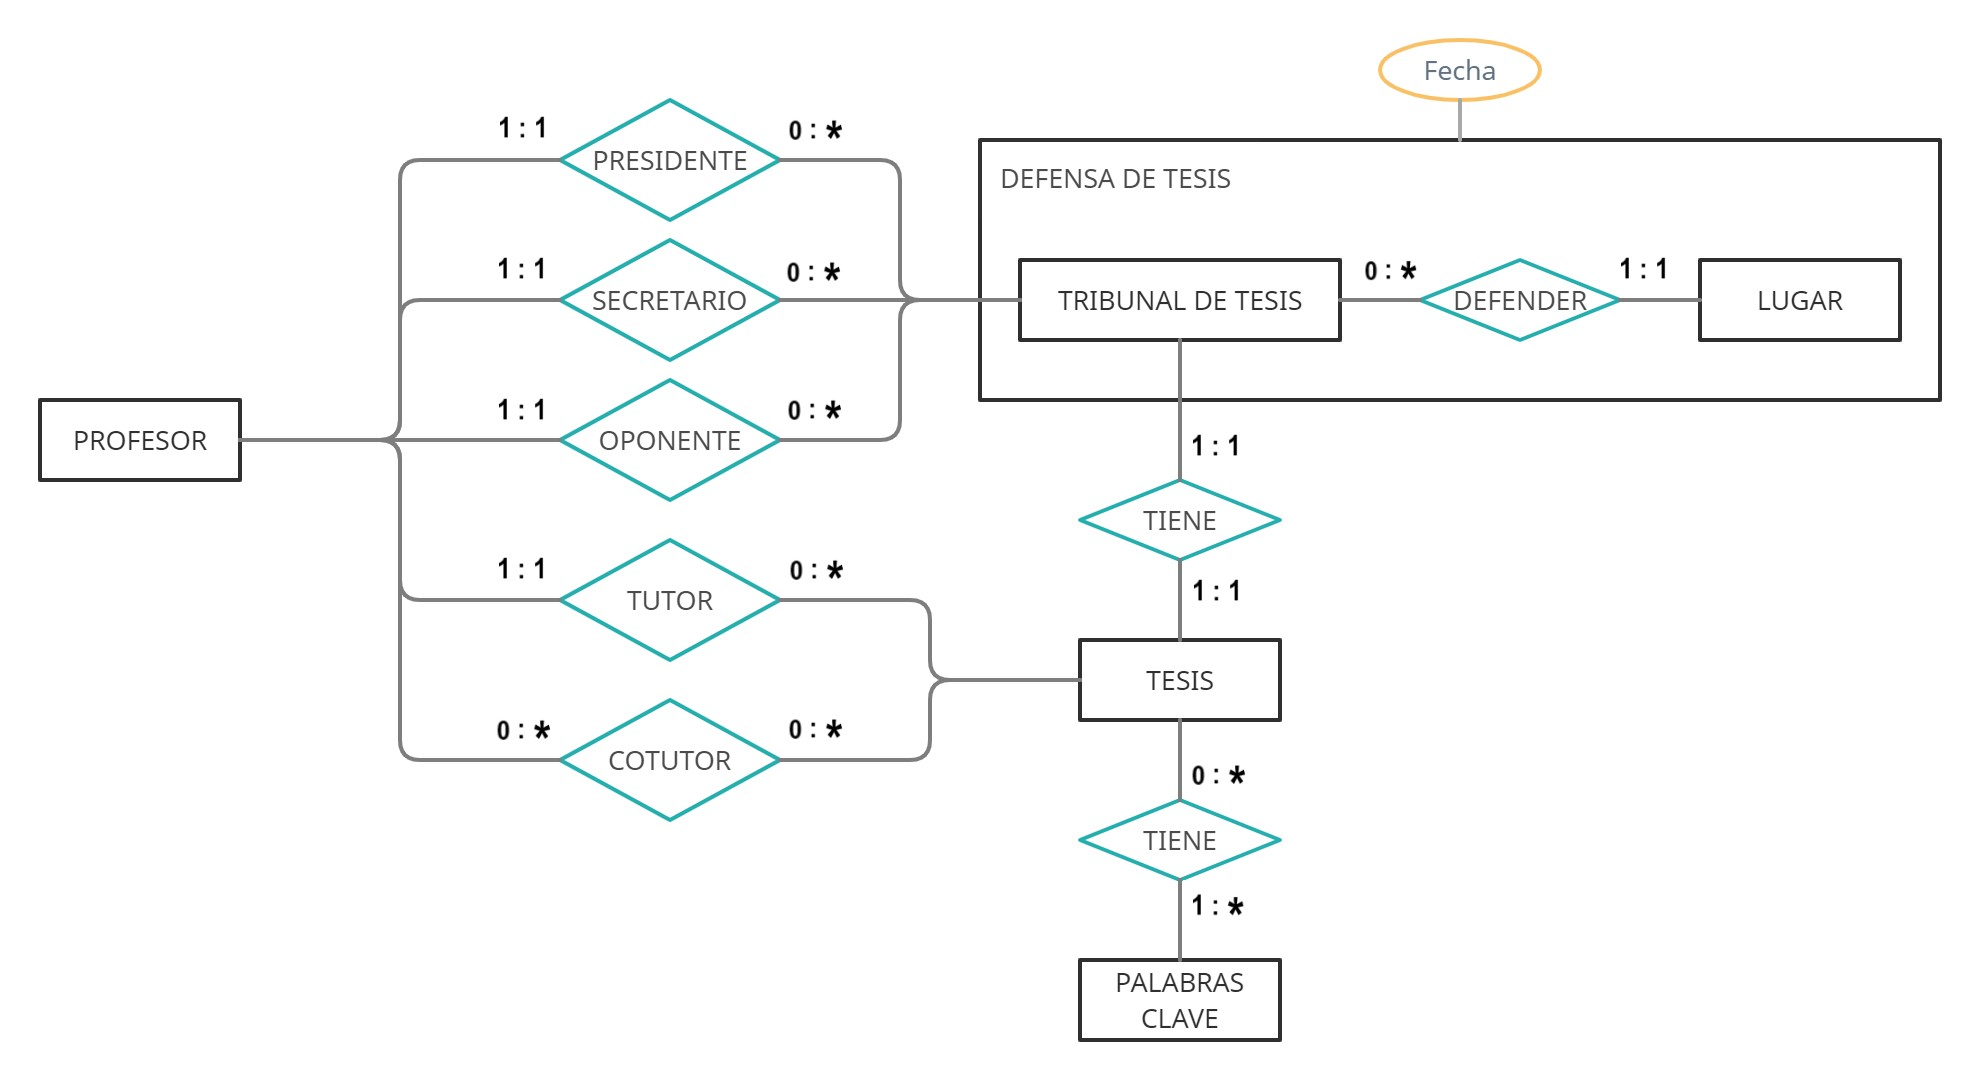
\includegraphics[scale=0.29]{Graphics/Database/MERXX-TC-FINAL.jpg}
\end{figure}


\subparagraph{TESIS:}
Agrupa los datos asociados a una tesis.
El título de la tesis y el autor se modelan como atributos, mientras que
el tutor, los cotutores y las palabras claves se modelan como relaciones con 
las entidades PROFESOR (tutor y cotutores) y PALABRAS CLAVES.
Una tesis tiene un único tutor, puede tener cero o muchos cotutores y tiene 
una o muchas palabras claves. 

\subparagraph{PALABRAS CLAVES:}
Representa las palabras claves que describen el contenido de una tesis.
El nombre o texto de las palabras claves se modela como un atributo. Una 
palabra clave puede aparecer en una o muchas tesis. 


\subparagraph{TRIBUNAL DE TESIS:}
Representa el tribunal de la defensa de una tesis.
Está compuesto por los miembros del tribunal: presidente, secretario y oponente, 
y la tesis, campos que se modelan como relaciones con las entidades PROFESOR y TESIS, respectivamente.
Un tribunal de tesis tiene una única tesis, un único presidente, un único secretario y 
un único oponente.


\subparagraph{DEFENSA DE TESIS:}
Representa el acto de defensa de la tesis. 
Está compuesta por un tribunal de tesis, en un local y una 
fecha determinada. La fecha se modela como un atributo mientras que 
el tribunal y el local se modelan como relaciones con las entidades TRIBUNAL DE 
TESIS y LOCAL, respectivamente. Una defensa de tesis tiene un único tribunal de tesis,
una única fecha y un único local.



\subparagraph{LOCAL:}
Representa el local donde se lleva a cabo la defensa de las tesis.
El nombre del local se modela como un atributo. 
En un local se puede realizar la defensa de cero o muchas tesis.


\subparagraph{PROFESOR:}
Se utiliza la misma entidad creada en el proceso de asignación de docencia.
Un profesor puede tener el rol de presidente, secretario u oponente en cero o 
muchos tribunales de tesis. Un profesor puede ser 
tutor o cotutor de cero o muchas tesis. \\


DESPUES DE LA MODELACION DE CADA PROCESO CREO Q DEBO HABLAR UN 
POCO DEL PROCESO DE NORMALIZACION PARA ESOS ESQUEMAS, Y REVISAR SI 
ESTAN EN 3FN... 

NO SE QUE MAS MENCIONAR EN ESTE CAPITULO.


